%----------------------------------------------------------------------------------------
%	PACKAGES AND DOCUMENT CONFIGURATIONS
%----------------------------------------------------------------------------------------

\documentclass[11pt,a4paper]{article}

\usepackage{graphicx} % Required for the inclusion of images
\usepackage{natbib} % Required to change bibliography style to APA
\usepackage{amsmath} % Required for some math elements 
\usepackage{subcaption}
\usepackage[justification=centering]{caption}
\usepackage[nomarkers,figuresonly,nofiglist]{endfloat}
\usepackage[margin=0.9in]{geometry}
\usepackage{sectsty}
\sectionfont{\fontsize{12}{15}\selectfont}
\setlength\parindent{0pt} % Removes all indentation from paragraphs
\usepackage{todonotes}
\usepackage{units} % for nice fractions \nicefrac{}{}
\usepackage[hidelinks=true]{hyperref}
\def\labelitemi{--}

\renewcommand{\labelenumi}{\alph{enumi}.} % Make numbering in the enumerate environment by letter rather than number

%%%%%%%%%% Start TeXmacs macros
\newcommand{\nocomma}{}
\newcommand{\noplus}{}
\newcommand{\tmop}[1]{\ensuremath{\operatorname{#1}}}
\newcommand{\upl}{+}
%%%%%%%%%% End TeXmacs macros

%----------------------------------------------------------------------------------------
%	DOCUMENT INFORMATION
%----------------------------------------------------------------------------------------

\title{Machine Translation Assignment 2: Decoding} % Title

\author{s0907677, s1520582} % Author name

\date{}

\begin{document}

\maketitle % Insert the title, author and date

\section*{Q1}
The default limitation of both stack size and maximum number of translation
to 1 is very restrictive and so one expects to see a significant improvement
in total log probability once either limit is increased. This proves to be
true, but only in a very limited range for both variables, as illustrated in
Figure~\ref{decode1}.
\vspace{4mm} %4mm vertical space

Changing the maximum number of translations causes a sharp improvement, but
it flattens out very quickly. The difference in total log probability
between decoder with $k=10$ and $k=50$ is only 10\% of the difference
between $k=1$ and $k=2$. No further improvements are observed for $k>50$.

Changing the stack size has a similar effect, although improvement tapers
out even quicker. Increasing stack size to over 3 does not provide
significant benefits.

Qualitatively, the difference between translations produced by the maximally
limited system ($k=1$ and $s=1$) and one which produces the highest scoring
output ($k=50$ and $s=10$) is that the latter text is more fluent and
idiomatic, yet the meaning is equally difficult to grasp and there is no
difference between the levels of syntactic correctness.

We did not investigate how parameter changes affect decoding speed. Simple
timing methods seemed to be neither sensitive nor reliable enough to uncover
any interesting trends for values of k and s in the range [1--100]. However,
Figure~\ref{swap} offers a decoding time comparison with the local reordering case. 
\vspace{4mm} %4mm vertical space

The following conclusions can be drawn:
\begin{enumerate}
	\item
    The intuitive insight that phrases can have multiple good translations,
    depending on the context, proves to be important. Increasing the maximum
    number of possible translations per phrase does improve output quality.
	\item
    The pruning heuristics used in decoding are justifiable, since the best
    translation can really be found by searching within the top few
    hypothesis in each stack. The best hypothesis is not always the very top
    one, as witnessed by the sharp increase in log probability when stack
    size is changed to 2, but it seems to almost always be one of the top 5
    or so.
	\item
    There is a limit, and one that's quickly reached, to how good a
    monotonic decoder can perform. Allowing it to entertain more hypotheses
    cannot overcome inherent problems entailed by monotonicity.
\end{enumerate}

\begin{figure}
	\centering
	\begin{subfigure}{.8\linewidth}
		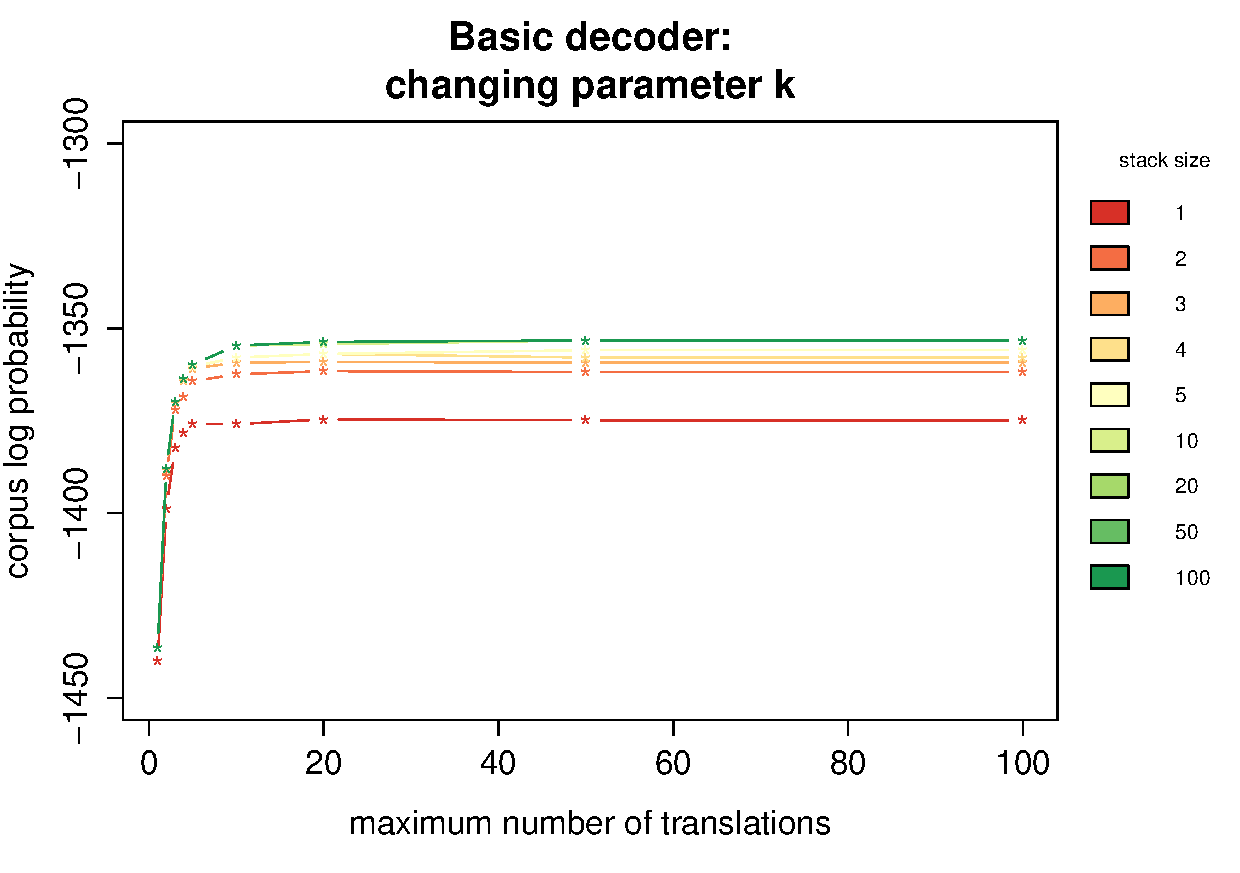
\includegraphics[scale=.65]{figures/d1_k.pdf}
		\caption{Increasing maximum number of translations, range [1--100].}
	\end{subfigure}
	\hskip2em
	\begin{subfigure}{.8\linewidth}
		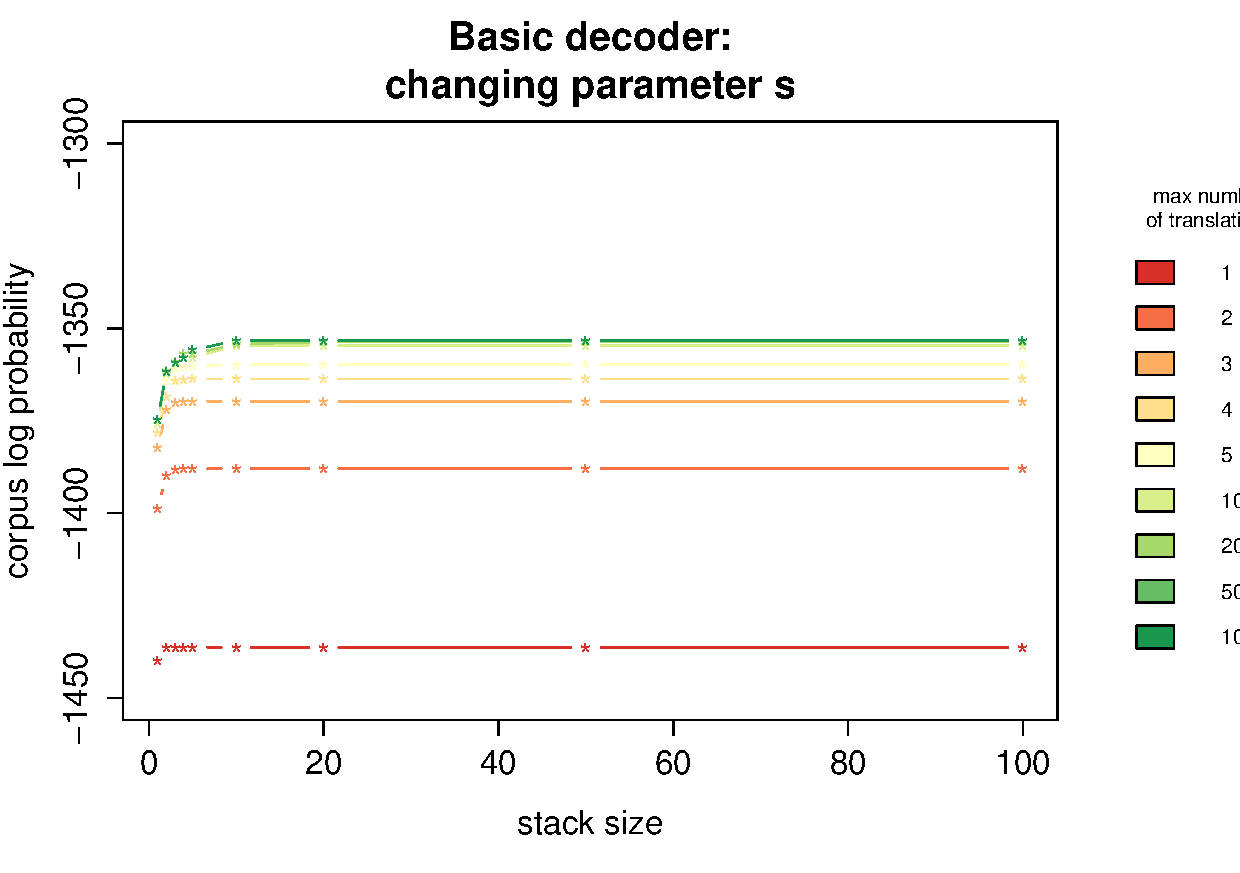
\includegraphics[scale=.65]{figures/d1_s.pdf}
		\caption{Increasing stack size, range [1--100].}
	\end{subfigure}
	\caption{Performance of decoder without reordering.}\label{decode1}
\end{figure}

\section*{Q2}
We modified the old $h(j,e)$ so that each recursion step reads two phrases
instead of one. The second of these phrases (in the French sentence) may be
the empty phrase $\varepsilon$. The two phrases are always swapped in the
translation. If the second phrase was $\varepsilon$, swapping has no effect
on the translation. Thus the translation is equivalent to a non-swap.
Our full definition of $h(j,e)$ is specified as follows:

$h (0 \nocomma, e) = \left\{ \begin{array}{l}
1 \nocomma, \tmop{if} \, e = \tmop{START}\\
0 \nocomma, \tmop{otherwise}
\end{array} \right.$
\begin{eqnarray}
h (j, e) = & \underset{h (i, e') e_1 \ldots e_k e_{k + 1} \ldots e_m
	e}{\tmop{argmax}}_{} & p (h (i, e')) \nonumber\\
& + & \log p_{\tmop{TM}} (f_{i + 1} \ldots f_c |e_{k + 1} \ldots e_m e)
\nonumber\\
& \noplus + & \log p_{\tmop{TM}} (f_{c + 1} \ldots f_j |e_1 \ldots e_k)
\nonumber\\
& \upl & \log p_{\tmop{LM}} (e_1 |e') + \sum_{k' = 1}^{m - 1} \log
p_{\tmop{LM}} (e_{k' + 1} |e_{k'}) + \log p_{\tmop{LM}} (e|e_m) \nonumber
\end{eqnarray}
with $0 \leq i < c \leq j$, $0 \leq k \leq m$, $e' \in V_E$, $e_1 \ldots e_k
\in t (f_{c + 1} \ldots f_j) \cup \{ \varepsilon \}$,\\
and $e_{k + 1} \ldots e_m e \in t (f_{i + 1} \ldots f_c)$.


\section*{Q3}
For each French sentence of length $n$, we loop over all $n$ possible stacks. In each stack, we look at the top $s$ hypotheses and expand them. To perform an expansion we choose two consecutive phrases (the second of which might be $\varepsilon$), swap them, and consider all possible combinations of the first $k$ translations of each phrase. The maximum considered length of phrase is $n$. Finally, the algorithm calculates the language model probability of the generated two-phrase translation. In this step, the algorithm has to iterate over up to $2 t$ words, where $t$ is the maximum length of a translation phrase. Thus the overall complexity is as follows:

\[
\mathcal{O}(n \cdot s) \cdot \mathcal{O}({(n \cdot k)}^2)
\cdot \mathcal{O}(t)
= \mathcal{O}(n^3 \cdot k^2 \cdot s \cdot t)
\]

\section*{Q4}

In our implementation the mapping from hypotheses to stacks is the same in the decoder with local reordering as it was in the one without. Each hypothesis is placed on a stack corresponding to the index of last French word being translated. We do not create hypotheses in which French phrases are skipped, but instead always look at two consecutive phrases, swap then, and create a hypothesis which covers both phrases. This means that mapping onto stacks is straightforward, since the number of French words covered by a hypothesis is always the same as the index of the last word which it translates.

\section*{Q5}

Our implementation of local reordering does not involve any changes to the hypotheses objects. We do modify the translation model by inserting into the dictionary an empty phrase, which translates to English with probability 1 as an empty string.

We introduce a modification in the hypothesis extension step. Given a hypothesis which ends at index \textit{i} in the French sentence we consider all indices \textit{c} and \textit{j} such that $c \leq j$, $j \leq sentence length$, and the fragments of the sentence delimited by \textit{[i, c]} and \textit{[c, j]} are phrases. Since we allow for $c = j$, the second phrase may be the empty one we have added to the translation model. For each discovered pair of phrases we create a hypothesis by swapping them and considering k best translations for each. For a pair with an empty phrase this amounts to no reordering. The hypotheses we generate do not have gaps in coverage of the source sentence and can be simply placed on the stack corresponding to the last word covered.

This approach provides for a simple implementation. We do not need to check if the hypothesis we are extending was or was not created by skipping a phrase. Each hypothesis we store was either created by reordering the last two phrases it covers, or by translating monotonically. In both cases we are free to reorder any next two consecutive phrases we find in the French sentence.


\section*{Q6}

Similarly to the non-reordering decoder, increases in the number of
translations $k$ lead to major improvements at first, but fewer improvements
$k>50$. In contrast to the results obtained from the simple decoder,
increases in the stack size $s$ do not fade out as quickly. The changes also
have a larger effect for smaller $s$, with the biggest difference between
$s=1$ and $s=2$. Even in the reordering decoder, we do not observe any
performance increases for $s>20$.

We note that $k$ and $s$ have a much larger effect on runtime than they have
for the simple decoder. Nonetheless, the run times of both decoders are
roughly similar (see Fig.~\ref{swaptime}). For $k = s = 10$, the sentences
are relatively well-formed, though still difficult to understand. Since we
are still using a bigram model, it is not surprising that long-term
dependencies are not correctly resolved.

\begin{figure}
	\centering
	\begin{subfigure}{.8\linewidth}
		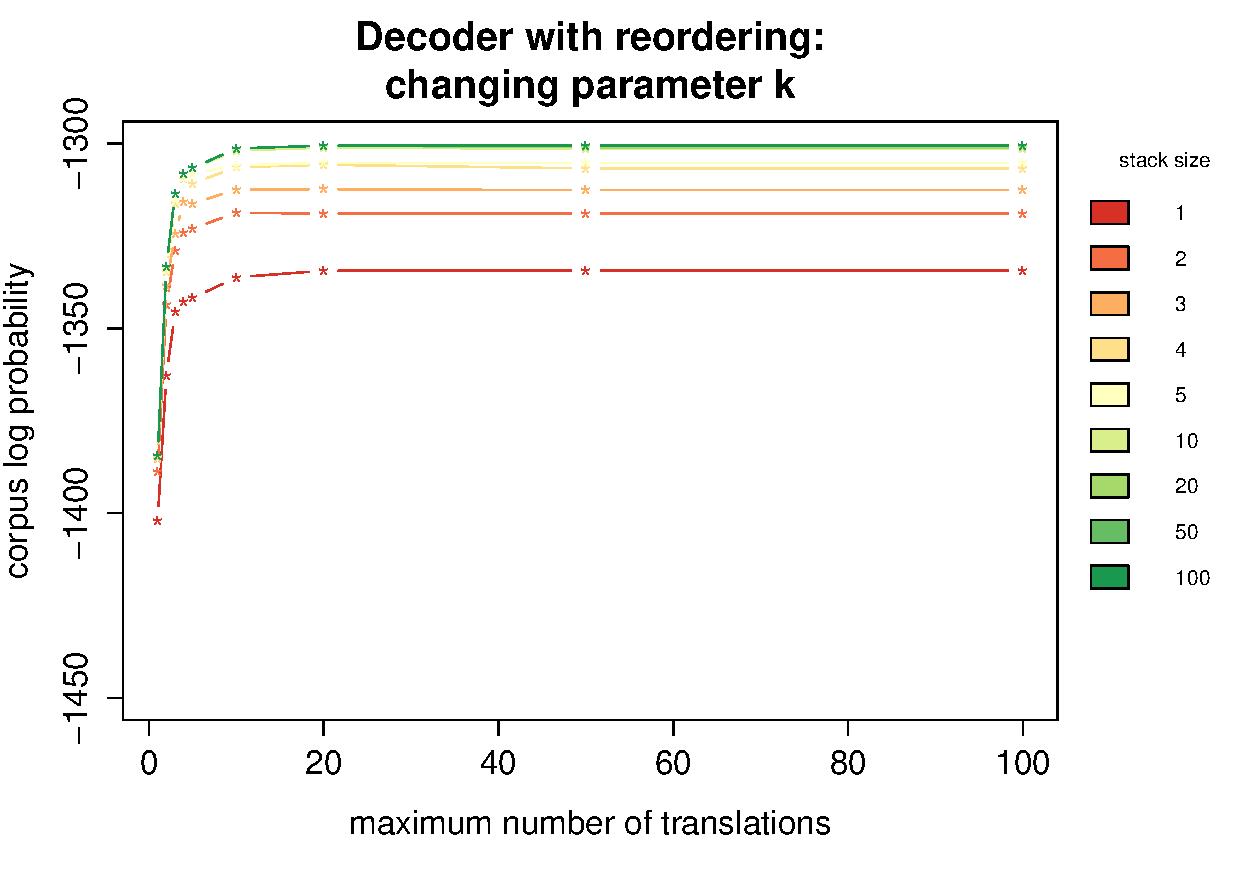
\includegraphics[scale=.65]{figures/d2_k.pdf}
		\caption{Increasing maximum number of translations, range [1--100].}
	\end{subfigure}
	\hskip2em
	\begin{subfigure}{.8\linewidth}
		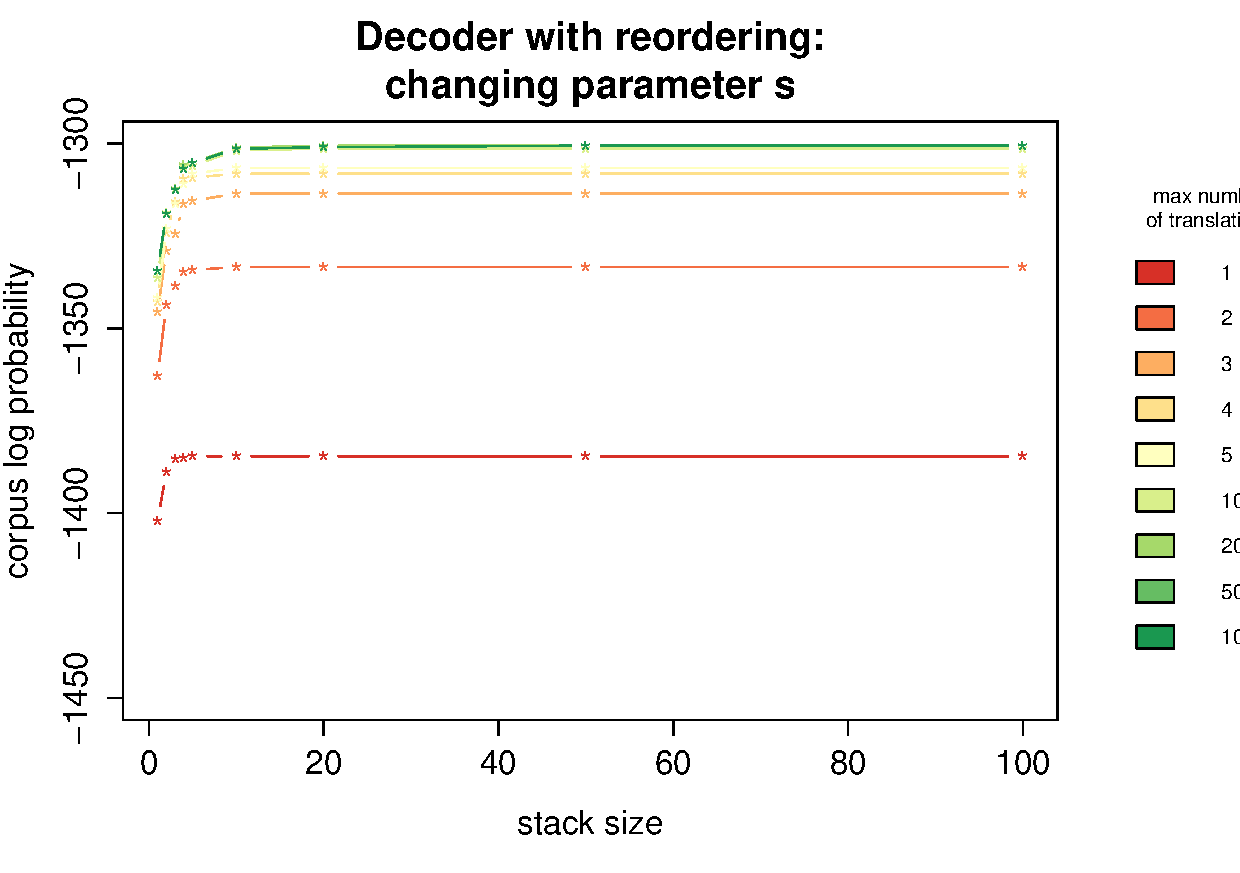
\includegraphics[scale=.65]{figures/d2_s.pdf}
		\caption{Increasing stack size, range [1--100].}
	\end{subfigure}
    \caption{Performance of decoder with local reordering.}\label{swap}
\end{figure}

\begin{figure}
	\centering
	\begin{subfigure}{.45\linewidth}
		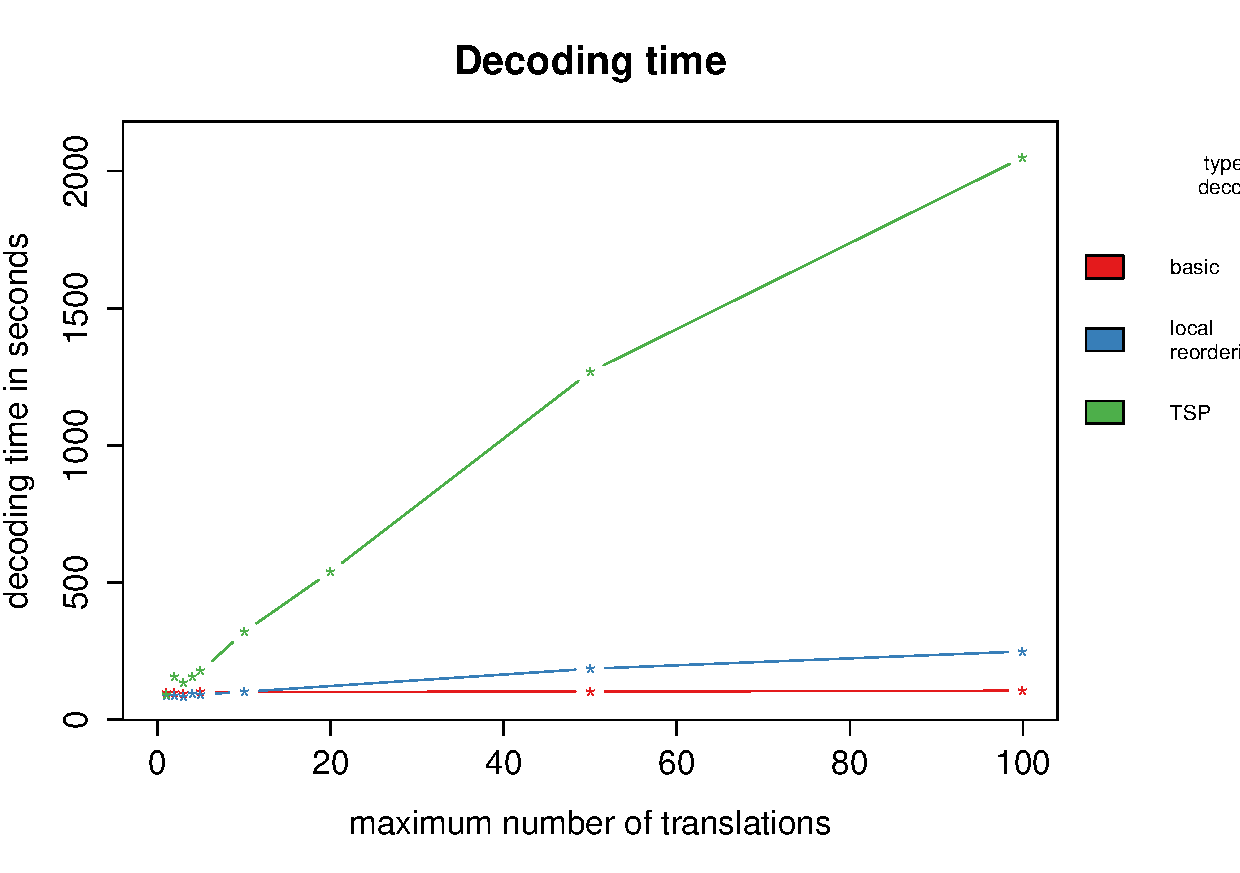
\includegraphics[scale=.35]{figures/time.pdf}
		\caption{Decoding time as function of maximum number of translations.}
	\end{subfigure}
	\hskip2em
	\begin{subfigure}{.45\linewidth}
		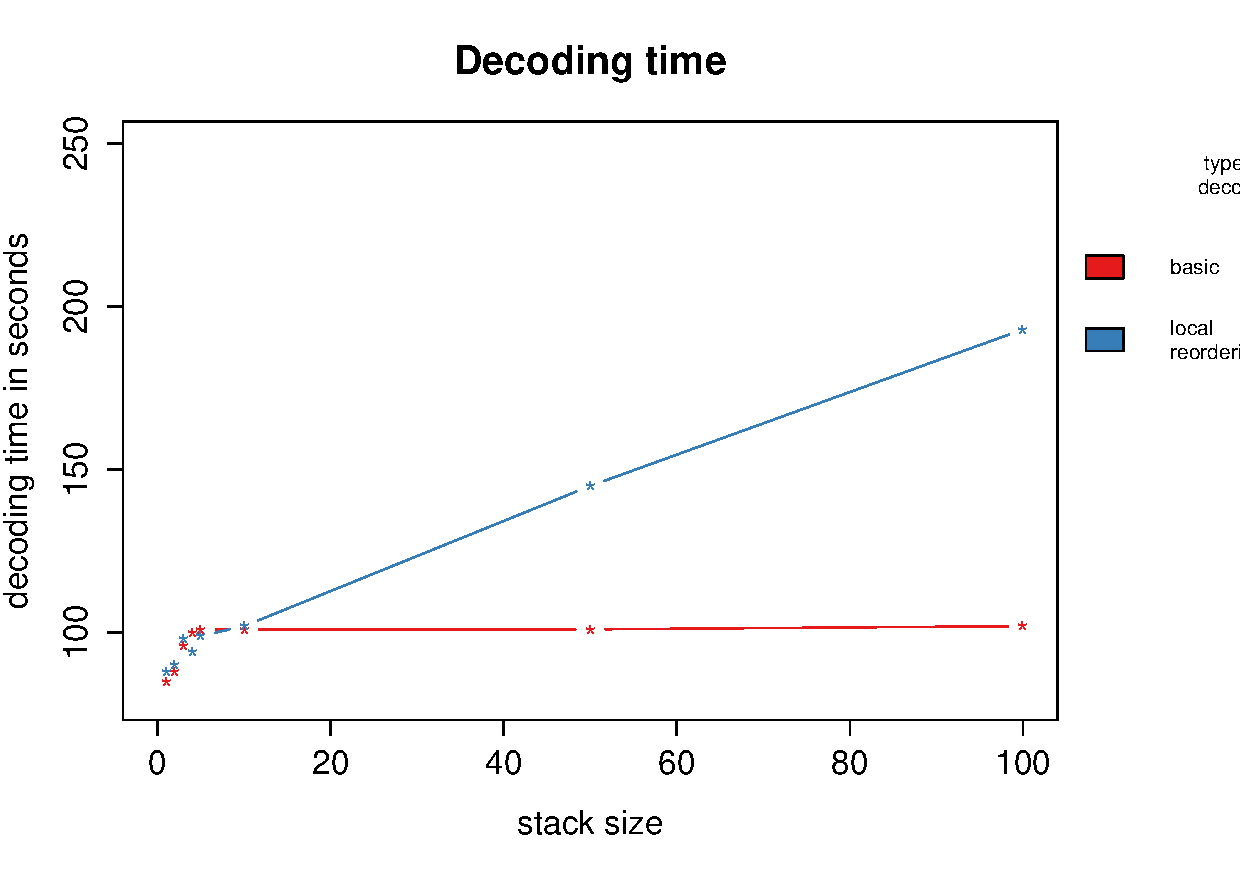
\includegraphics[scale=.35]{figures/time_d1_d2.pdf}
		\caption{Decoding time as a function of stack size.}
	\end{subfigure}
	\caption{Decoding time for the three decoders.}\label{swaptime}
\end{figure}


\section*{Q7}

We based our decoder on the correspondence between phrase-based decoding and
the Traveling Salesman Problem, following the proposal
of~\cite{zaslavskiy2009}.

Our implementation includes the following steps:
\begin{enumerate}
    \item project the translation problem to an \emph{Asymmetric Generalized
        Travelling Salesman Problem} [\textsc{AGTSP}].
    \item convert the \textsc{AGTSP} to an \emph{Asymmetric Travelling
        Salesman Problem} [\textsc{ATSP}].
    \item find the best path by utilizing the LKH package implementation of the
        Lin-Kernighan~heuristic~\cite{Helsgaun2006}\footnote{http://www.akira.ruc.dk/~keld/research/LKH/}.
\end{enumerate}

We transform a sentence into an asymmetric graph by following the procedure
described in~\cite{zaslavskiy2009}: We extract all possible phrases from the
French sentence. For each phrase we retrieve $k$ possible translations and
store the possible pairs as a biphrase each. For each combination of a French word in the
phrase and an English biphrase, we create a node (word, biphrase) in the
\textsc{AGTSP} graph. Nodes sharing the same French word form a group. In
\textsc{AGTSP}, each group has to be visited once. This means that the
algorithm forces us to cover each French word with a phrase. We decide on
costs for each directed edge following the approach described in the
article: Edges within a phrase carry zero costs, whereas the cost of prase
transitions is determined by the translation model cost and language model
cost of the phrase we connect to and the distance of the connected words in
the French phrase.

We have to convert our \textsc{AGTSP} to an \textsc{ATSP} so that we can use
the solver by~\cite{Helsgaun2006}. This projection is done in polynomial
time and converts each group to a directed cycle of nodes with large
negative weights. The exact conversion is described in the article.

The original article optimizes three parameters to weigh the relative
importance of translation model, language model, and phrase distance.
We simplified the model by setting these parameters to constant 1. Secondly,
we do not use the exact \emph{concorde} \textsc{TSP} solver. Instead, we use
an heuristical solver which can operate on the directed \textsc{ATSP}s.

The proposed model does not reach the same translation quality as the
default non-swapping decoder, as measured by \texttt{compute-model-score}.
A possible difficulty lies in the fact that our edge costs are calculated in
advance, so that our language model has only a limited context to work on.
This is especially a problem for one-word phrases which consist of
out-of-dictionary words.

TODO


%----------------------------------------------------------------------------------------
%	BIBLIOGRAPHY
%----------------------------------------------------------------------------------------
\bibliographystyle{apalike}

\bibliography{bibliography}

%----------------------------------------------------------------------------------------


\end{document}
